\documentclass[a4paper]{article}

\usepackage{inputenc}
\usepackage[british,UKenglish]{babel}
\usepackage{amsmath}
%\usepackage{titlesec}
\usepackage{color}
\usepackage{graphicx}
\usepackage{fancyref}
\usepackage{hyperref}
\usepackage{float}
\usepackage{scrextend}
\usepackage{setspace}
\usepackage{xargs}
\usepackage{multicol}
\usepackage{nameref}

\usepackage{sectsty}
\usepackage{multicol}
\usepackage{multirow}
\usepackage[procnames]{listings}
\usepackage{appendix}

\newcommand\tab[1][1cm]{\hspace*{#1}}
\hypersetup{colorlinks=true, linkcolor=black}
\interfootnotelinepenalty=10000

\newcommand{\cleancode}[1]{\begin{addmargin}[3em]{3em}\texttt{\textcolor{cleanOrange}{#1}}\end{addmargin}}
\newcommand{\cleanstyle}[1]{\text{\textcolor{cleanOrange}{\texttt{#1}}}}


\usepackage[colorinlistoftodos,prependcaption,textsize=footnotesize]{todonotes}
\newcommandx{\commred}[2][1=]{\textcolor{Red}
{\todo[linecolor=red,backgroundcolor=red!25,bordercolor=red,#1]{#2}}}
\newcommandx{\commblue}[2][1=]{\textcolor{Blue}
{\todo[linecolor=blue,backgroundcolor=blue!25,bordercolor=blue,#1]{#2}}}
\newcommandx{\commgreen}[2][1=]{\textcolor{OliveGreen}{\todo[linecolor=OliveGreen,backgroundcolor=OliveGreen!25,bordercolor=OliveGreen,#1]{#2}}}
\newcommandx{\commpurp}[2][1=]{\textcolor{Plum}{\todo[linecolor=Plum,backgroundcolor=Plum!25,bordercolor=Plum,#1]{#2}}}

\def\code#1{{\tt #1}}

\def\note#1{\noindent{\bf [Note: #1]}}

\makeatletter
%% The "\@seccntformat" command is an auxiliary command
%% (see pp. 26f. of 'The LaTeX Companion,' 2nd. ed.)
\def\@seccntformat#1{\@ifundefined{#1@cntformat}%
   {\csname the#1\endcsname\quad}  % default
   {\csname #1@cntformat\endcsname}% enable individual control
}
\let\oldappendix\appendix %% save current definition of \appendix
\renewcommand\appendix{%
    \oldappendix
    \newcommand{\section@cntformat}{\appendixname~\thesection\quad}
}
\makeatother


% "define" Scala
\usepackage[T1]{fontenc}  
\usepackage[scaled=0.82]{beramono}  
\usepackage{microtype} 

\sbox0{\small\ttfamily A}
\edef\mybasewidth{\the\wd0 }

\lstdefinelanguage{scala}{
  morekeywords={abstract,case,catch,class,def,%
    do,else,extends,false,final,finally,%
    for,if,implicit,import,match,mixin,%
    new,null,object,override,package,%
    private,protected,requires,return,sealed,%
    super,this,throw,trait,true,try,%
    type,val,var,while,with,yield},
  sensitive=true,
  morecomment=[l]{//},
  morecomment=[n]{/*}{*/},
  morestring=[b]",
  morestring=[b]',
  morestring=[b]"""
}

\usepackage{color}
\definecolor{dkgreen}{rgb}{0,0.6,0}
\definecolor{gray}{rgb}{0.5,0.5,0.5}
\definecolor{mauve}{rgb}{0.58,0,0.82}

% Default settings for code listings
\lstset{frame=tb,
  language=scala,
  aboveskip=3mm,
  belowskip=3mm,
  showstringspaces=false,
  columns=fixed, % basewidth=\mybasewidth,
  basicstyle={\small\ttfamily},
  numbers=none,
  numberstyle=\footnotesize\color{gray},
  % identifierstyle=\color{red},
  keywordstyle=\color{blue},
  commentstyle=\color{dkgreen},
  stringstyle=\color{mauve},
  frame=single,
  breaklines=true,
  breakatwhitespace=true,
  procnamekeys={def, val, var, class, trait, object, extends},
  procnamestyle=\ttfamily\color{red},
  tabsize=2
}

\lstnewenvironment{scala}[1][]
{\lstset{language=scala,#1}}
{}
\lstnewenvironment{cpp}[1][]
{\lstset{language=C++,#1}}
{}
\lstnewenvironment{bash}[1][]
{\lstset{language=bash,#1}}
{}
\lstnewenvironment{verilog}[1][]
{\lstset{language=verilog,#1}}
{}



%代码段设置
\lstset{numbers=left,
basicstyle=\tiny,
numberstyle=\tiny,
keywordstyle=\color{blue!70},
commentstyle=\color{red!50!green!50!blue!50},
frame=single, rulesepcolor=\color{red!20!green!20!blue!20},
escapeinside=``
}

\graphicspath{ {figures/} }
\usepackage{ctex}
\setCJKmainfont[ItalicFont=Noto Sans CJK SC Bold, BoldFont=Noto Serif CJK SC Black]{Noto Serif CJK SC}
\usepackage{graphicx}
\usepackage{color,framed}%文本框
\usepackage{listings}
\usepackage{caption}
\usepackage{amssymb}
\usepackage{enumerate}
\usepackage{xcolor}
\usepackage{bm} 
\usepackage{lastpage}%获得总页数
\usepackage{fancyhdr}
\usepackage{tabularx}  
\usepackage{geometry}
\usepackage{minted}
\usepackage{graphics}
\usepackage{subfigure}
\usepackage{float}
\usepackage{pdfpages}
\usepackage{pgfplots}
\pgfplotsset{width=10cm,compat=1.9}
\usepackage{multirow}
\usepackage{footnote}
\usepackage{booktabs}

%-----------------------伪代码------------------
\usepackage{algorithm}  
\usepackage{algorithmicx}  
\usepackage{algpseudocode}  
\floatname{algorithm}{Algorithm}  
\renewcommand{\algorithmicrequire}{\textbf{Input:}}  
\renewcommand{\algorithmicensure}{\textbf{Output:}} 
\usepackage{lipsum}  
\makeatletter
\newenvironment{breakablealgorithm}
  {% \begin{breakablealgorithm}
  \begin{center}
     \refstepcounter{algorithm}% New algorithm
     \hrule height.8pt depth0pt \kern2pt% \@fs@pre for \@fs@ruled
     \renewcommand{\caption}[2][\relax]{% Make a new \caption
      {\raggedright\textbf{\ALG@name~\thealgorithm} ##2\par}%
      \ifx\relax##1\relax % #1 is \relax
         \addcontentsline{loa}{algorithm}{\protect\numberline{\thealgorithm}##2}%
      \else % #1 is not \relax
         \addcontentsline{loa}{algorithm}{\protect\numberline{\thealgorithm}##1}%
      \fi
      \kern2pt\hrule\kern2pt
     }
  }{% \end{breakablealgorithm}
     \kern2pt\hrule\relax% \@fs@post for \@fs@ruled
  \end{center}
  }
\makeatother
%------------------------代码-------------------
\usepackage{xcolor} 
\usepackage{listings} 
\lstset{ 
breaklines,%自动换行
basicstyle=\small,
escapeinside=``,
keywordstyle=\color{ blue!70} \bfseries,
commentstyle=\color{red!50!green!50!blue!50},% 
stringstyle=\ttfamily,% 
extendedchars=false,% 
linewidth=\textwidth,% 
numbers=left,% 
numberstyle=\tiny \color{blue!50},% 
frame=trbl% 
rulesepcolor= \color{ red!20!green!20!blue!20} 
}

%-------------------------页面边距--------------
\geometry{a4paper,left=2.3cm,right=2.3cm,top=2.7cm,bottom=2.7cm}
%-------------------------页眉页脚--------------
\usepackage{fancyhdr}
\pagestyle{fancy}
\lhead{\kaishu \leftmark}
% \chead{}
\rhead{\kaishu 并行程序设计实验报告}%加粗\bfseries 
\lfoot{}
\cfoot{\thepage}
\rfoot{}
\renewcommand{\headrulewidth}{0.1pt}  
\renewcommand{\footrulewidth}{0pt}%去掉横线
\newcommand{\HRule}{\rule{\linewidth}{0.5mm}}%标题横线
\newcommand{\HRulegrossa}{\rule{\linewidth}{1.2mm}}
\setlength{\textfloatsep}{10mm}%设置图片的前后间距
%--------------------文档内容--------------------

\begin{document}
\renewcommand{\contentsname}{目\ 录}
\renewcommand{\appendixname}{附录}
\renewcommand{\appendixpagename}{附录}
\renewcommand{\refname}{参考文献}
\renewcommand{\figurename}{图}
\renewcommand{\tablename}{表}
\renewcommand{\today}{\number\year 年 \number\month 月 \number\day 日}

%-------------------------封面----------------
\begin{titlepage}
  \begin{center}
    
\includegraphics[width=0.8\textwidth]{NKU.png}\\[1cm]
    \vspace{20mm}
    \textbf{\huge\textbf{\kaishu{计算机学院}}}\\[0.5cm]
    \textbf{\huge{\kaishu{并行程序设计第 6 次作业}}}\\[2.3cm]
    \textbf{\Huge\textbf{\kaishu{高斯消去法的 CUDA 并行化}}}

    \vspace{\fill}

    % \textbf{\Large \textbf{并行程序设计期末实验报告}}\\[0.8cm]
    % \HRule \\[0.9cm]
    % \HRule \\[2.0cm]
    \centering
    \textsc{\LARGE \kaishu{姓名\ :\ 丁屹}}\\[0.5cm]
    \textsc{\LARGE \kaishu{学号\ :\ 2013280}}\\[0.5cm]
    \textsc{\LARGE \kaishu{专业\ :\ 计算机科学与技术}}\\[0.5cm]

    \vfill
    {\Large \today}
  \end{center}
\end{titlepage}

\renewcommand {\thefigure}{\thesection{}.\arabic{figure}}%图片按章标号
\renewcommand{\figurename}{图}
\renewcommand{\contentsname}{目录}
\cfoot{\thepage\ of \pageref{LastPage}}%当前页 of 总页数


% 生成目录
\clearpage
\tableofcontents
\newpage

\section{问题描述}
高斯消去的计算模式如图 \ref{gauss} 所示,在第$k$步时,对第$k$行从$(k, k)$开始进行除法操作,并且将后续的$k + 1$至$N$行进行减去第$k$行的操作,串行算法如下面伪代码所示。
\begin{figure}
  \centering
  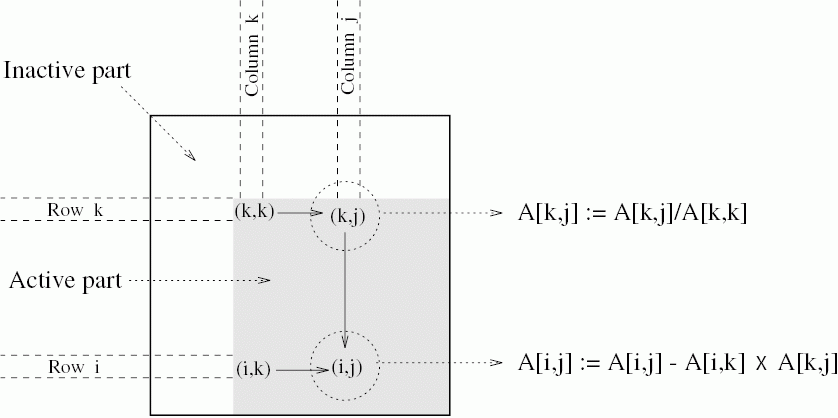
\includegraphics[width=1\textwidth]{gauss.png}
  \caption{高斯消去法示意图}
  \label{gauss}
\end{figure}
\begin{breakablealgorithm}
  \caption{普通高斯消元算法伪代码}
  \begin{algorithmic}[1] %每行显示行号  
    \Function {LU}{}
    \For {$k:=0$\ \textbf{to}\ $n$}
    \For {$j:=k+1$\ \textbf{to}\ $n$}
    \State {$A[k,j]:=A[k,j]/A[k,k]$}
    \EndFor
    \State{$A[k,k]:=1.0$}
    \For {$i:=k+1$\ \textbf{to}\ $n$}
    \For {$j:=k+1$\ \textbf{to}\ $n$}
    \State {$A[i,j]:=A[i,j]-A[i,k]*A[k,j]$}
    \EndFor
    \State{$A[i,k]:=0$}
    \EndFor
    \EndFor
    \EndFunction
  \end{algorithmic}
\end{breakablealgorithm}

观察高斯消去算法,注意到伪代码第 4,5 行第一个内嵌循环中的$A[k, j] := A[k, j]/A[k, k]$以及伪代码第$8,9,10$行双层$for$循环中的$A[i, j] := A[i, j] − A[i, k]×A[k, j]$都是可以进行向量化的循环。可以通过 CUDA 对这两步进行并行优化。

\section{算法设计}

源码链接:
\url{https://github.com/ArcanusNEO/Parallel-Programming/tree/master/6}

\subsection{测试用例的确定}

由于测试数据集较大,不便于各个平台同步,所以采用固定随机数种子为 $12345687$ 的 mt19937随机数生成器。
经过实验发现不同规模下,所有元素独立生成,限制大小在 $[0, 100]$,能够生成可以被正确消元的矩阵。

代码如下:

\begin{lstlisting}[frame=trbl,language={C++}]
  uniform_real_distribution<float> dist(0, 100);
  mt19937       mt(12345687);
  int           n;
  istringstream iss(argv[1]);
  iss >> n;
  cout << n << endl;
  for (int i = 1; i <= n; ++i)
    for (int j = 1; j <= n; ++j) cout << dist(mt) << " \n"[j == n];
\end{lstlisting}

\subsection{实验环境和相关配置}

实验在本地 Arch Linux x86\_64 平台完成,使用 cmake 构建项目,均开启 O3 加速;

\begin{itemize}
  \item nVIDIA GPU 型号:NVIDIA GeForce RTX 2060 with Max-Q Design
  \item 驱动版本:Driver Version: 515.48.07
  \item CUDA 版本:CUDA Version: 11.7
\end{itemize}

\subsection{默认平凡算法}

使用一维数组模拟矩阵,避免改变矩阵大小时第二维不方便调整、必须设成最大值的问题,可以减少 cache 失效;

使用 $\#define\ matrix(i, j)\ arr[(i) * n + (j)]$ 宏,增强可读性;

\begin{lstlisting}[frame=trbl,language={C++}]
void func(int& ans, float arr[], int n) {
  for (int k = 0; k < n; ++k) {
    for (int j = k + 1; j < n; ++j) matrix(k, j) = matrix(k, j) / matrix(k, k);
    matrix(k, k) = 1.0;
    for (int i = k + 1; i < n; ++i) {
      for (int j = k + 1; j < n; ++j)
        matrix(i, j) = matrix(i, j) - matrix(i, k) * matrix(k, j);
      matrix(i, k) = 0;
    }
  }
}
\end{lstlisting}

\subsection{CUDA 加速算法}
对于访存,这里使用了基本的内存空间分配方式,即在 CPU 端给数据分配好内存空间并初始化以后,在 GPU 端对应地分配显存空间,然后显式地调用数据传输的接口将 CPU 端的数据传输至 GPU 端;最后,核函数执行完毕后,还需要把计算好的数据再从 GPU 端传输回来。

对于任务划分,使用了最简单直观的任务划分方法:除法和消去部分串行执行,分别编写两个核函数。

对于除法部分,每个线程负责第 K 次循环中单独一列的计算,因为通过 cudaDeviceProp::maxThreadsPerBlock 可以发现在我的显卡上每个线程块的最大线程数为 1024,所以对于大于 1024 × 1024 的矩阵可以分成多个块并行执行。

\begin{lstlisting}[frame=trbl,language={C++}]
__global__ void division_kernel(float arr[], int n, int k) {
  auto tid = blockDim.x * blockIdx.x + threadIdx.x;
  if (k < tid && tid < n) matrix(k, tid) /= matrix(k, k);
}
\end{lstlisting}

对于消去部分,在第 k 次循环中,对第 k + 1 行至最后一行进行消去,每一行计算完成后需要将这一行的第 k 列设为 0,矩阵最后变为一个上三角矩阵。对于同步问题,在核函数内部调用 \_\_syncthreads() 接口来同步块内线程,但是 GPU 的硬件架构导致的没有接口用于块间同步,所以为了保证正确同步的同时最大化利用 GPU 的并行性,我们让一个线程块负责固定一行的计算任务,块内的线程分别负责这一行的不同位置上的元素的运算任务,最后进行块内同步。

\begin{lstlisting}[frame=trbl,language={C++}]
__global__ void eliminate_kernel(float arr[], int n, int k) {
  auto tx = blockDim.x * blockIdx.x + threadIdx.x;
  if (tx == 0) matrix(k, k) = 1.0;
  for (auto row = k + 1 + blockIdx.x; row < n; row += gridDim.x) {
    auto tid = threadIdx.x;
    for (auto col = k + 1 + tid; col < n; col += blockDim.x)
      matrix(row, col) -= matrix(row, k) * matrix(k, col);
    __syncthreads();
    if (tid == 0) matrix(row, k) = 0;
  }
}
\end{lstlisting}

在外层通用驱动程序 func 中,我们需要做的工作如下:
\begin{enumerate}
  \item 分配合适大小的显存
  \item 把内存中的矩阵复制进显存
  \item 对外层循环的每一轮确定合适的线程块大小和线程块数量
  \item 在外层循环的每一轮中依次调用 division\_kernel 和 eliminate\_kernel 函数并同步所有线程
  \item 把显存中的结果复制回内存,释放显存
\end{enumerate}

\begin{lstlisting}[frame=trbl,language={C++}]
void func(int& ans, float arr[], int n) {
  float* gpu_arr;
  auto   siz = sizeof(float) * n * n;
  if (cudaMalloc(&gpu_arr, siz) != cudaSuccess)
    cerr << "cudaMalloc failed" << endl;
  if (cudaMemcpy(gpu_arr, arr, siz, cudaMemcpyHostToDevice) != cudaSuccess)
    cerr << "cudaMemcpyHostToDevice failed" << endl;

  for (int k = 0; k < n; ++k) {
    auto rest = n - k - 1;
    dim3 grid(std::max(std::ceil(rest / 1024.0), 1.0));
    dim3 block(1024);
    division_kernel<<<grid, block>>>(gpu_arr, n, k);
    cudaDeviceSynchronize();
    if (auto ret = cudaGetLastError(); ret != cudaSuccess)
      cerr << "division kernel failed: " << cudaGetErrorString(ret) << endl;
    dim3 eliminate_grid(32);
    eliminate_kernel<<<eliminate_grid, block>>>(gpu_arr, n, k);
    cudaDeviceSynchronize();
    if (auto ret = cudaGetLastError(); ret != cudaSuccess)
      cerr << "eliminate kernel failed: " << cudaGetErrorString(ret) << endl;
  }
  if (cudaMemcpy(arr, gpu_arr, siz, cudaMemcpyDeviceToHost) != cudaSuccess)
    cerr << "cudaMemcpyDeviceToHost failed" << endl;
  cudaFree(gpu_arr);
}
\end{lstlisting}

\section{结果分析}

使用 GPU 加速需要考虑到浮点数精度的问题,在 solve.cc 文件内有一段被注释的代码控制打印结果矩阵,四舍五入保留 4 位小数。比较 8 × 8 矩阵的计算结果图 \ref{pic:ord8} 和 \ref{pic:cuda8} 发现二者结果完全一致;比较 16 × 16 矩阵的计算结果图 \ref{pic:ord16} 和 \ref{pic:cuda16} 发现某些元素最后一位小数略有差异。

\begin{figure}[h]
  \centering
  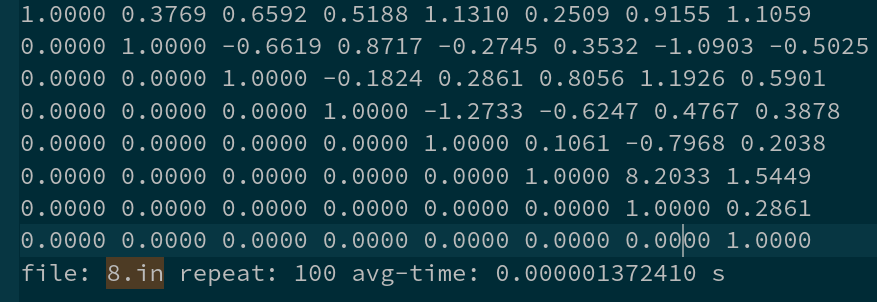
\includegraphics[width=\textwidth]{ord8.png}
  \caption{CPU 平凡算法 8 × 8 矩阵结果}
  \label{pic:ord8}
\end{figure}

\begin{figure}[h]
  \centering
  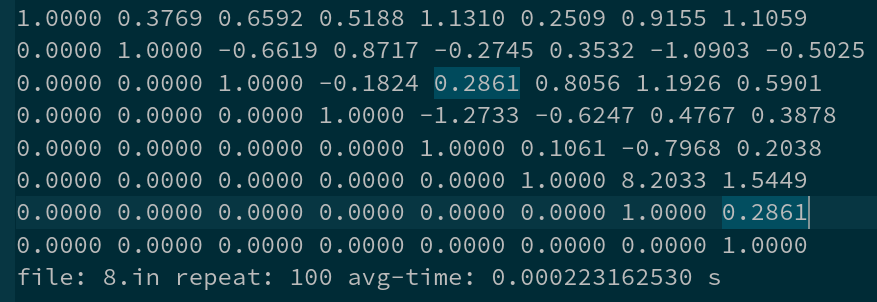
\includegraphics[width=\textwidth]{cuda8.png}
  \caption{GPU CUDA 加速算法 8 × 8 矩阵结果}
  \label{pic:cuda8}
\end{figure}

\begin{figure}[h]
  \centering
  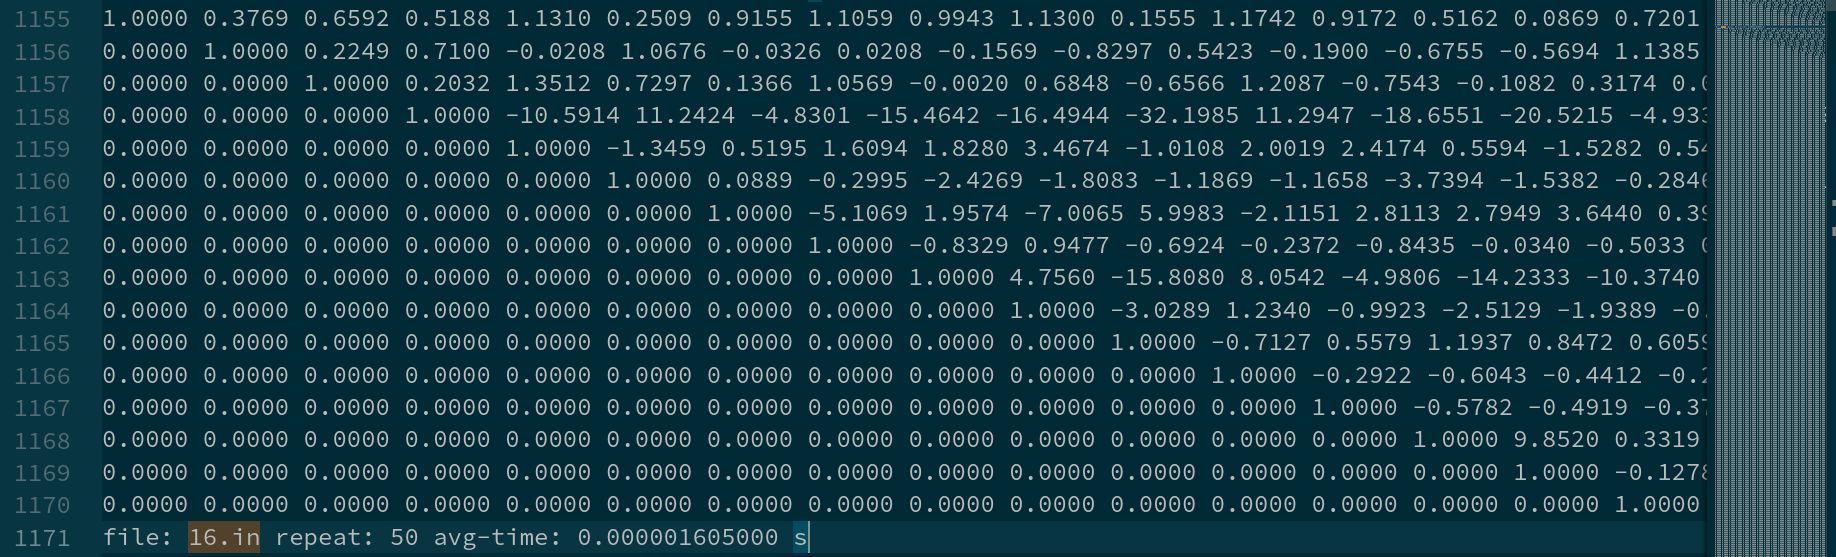
\includegraphics[width=\textwidth]{ord16.png}
  \caption{CPU 平凡算法 16 × 16 矩阵结果}
  \label{pic:ord16}
\end{figure}

\begin{figure}[h]
  \centering
  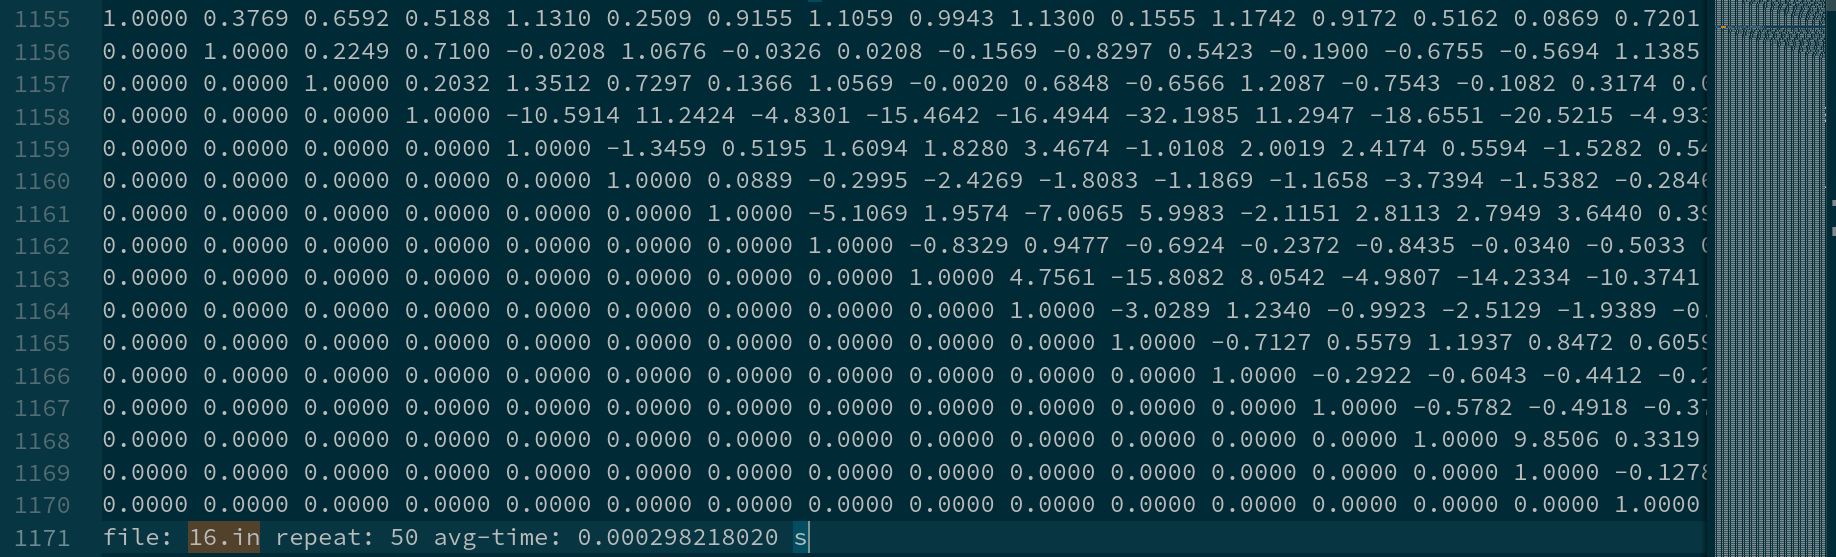
\includegraphics[width=\textwidth]{cuda16.png}
  \caption{GPU CUDA 加速算法 16 × 16 矩阵结果}
  \label{pic:cuda16}
\end{figure}

经过测试得到表 \ref{tab:ord-cuda} 发现大数据规模下 CUDA 加速效果显著,有十余倍性能提升。

\begin{table}[]
  \centering
  \resizebox{\textwidth}{!}{%
    \begin{tabular}{|ll|ll|}
      \hline
      Scale       & Reperat times & x86 ordinary (s) & x86 CUDA (s)   \\ \hline
      8×8         & 100           & 0.000001330460   & 0.000202092680 \\ \hline
      16 × 16     & 50            & 0.000001706920   & 0.000348178360 \\ \hline
      32 × 32     & 50            & 0.000003640080   & 0.000486327180 \\ \hline
      64 × 64     & 20            & 0.000015253300   & 0.000934846400 \\ \hline
      128 × 128   & 15            & 0.000098880800   & 0.002263211200 \\ \hline
      256 × 256   & 10            & 0.000716408500   & 0.003708655900 \\ \hline
      512 × 512   & 10            & 0.006722607300   & 0.008892275300 \\ \hline
      1024 × 1024 & 5             & 0.064893815400   & 0.054395600600 \\ \hline
      2048 × 2048 & 3             & 1.400074583333   & 0.240155499000 \\ \hline
      4096 × 4096 & 1             & 10.705585484000  & 1.255606927000 \\ \hline
    \end{tabular}%
  }
  \caption{平凡算法和 CUDA 加速算法运行时间}
  \label{tab:ord-cuda}
\end{table}

% \newpage

% \section{参考文献}
% \cite{1}\cite{2}\cite{3}\cite{4}\cite{5}\cite{6}

% \bibliographystyle{plain}
% \bibliography{Parallel-Programming-0.bib}

\end{document}